\newcommand{\fwb}{2.45cm}  % width
\newcommand{\fwh}{1.6cm}     % height
\begin{figure}[t]
\centering
%\begin{tabular}{C{\fwb}C{\fwb}C{\fwb}}
\begin{tabular}{ccc}
%kernel & draws from GP & GP posterior \\
\rotatebox{90}{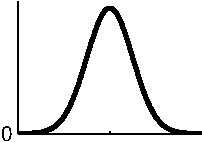
\includegraphics[width=\fwh,height=\fwb]{figures/structure_examples/se_kernel}} &  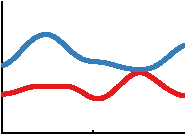
\includegraphics[width=\fwb,height=\fwh]{figures/structure_examples/se_kernel_draws} & 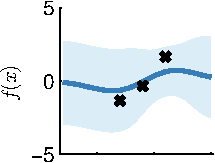
\includegraphics[width=\fwb,height=\fwh]{figures/structure_examples/se_kernel_post} \\
squared-exp & \multicolumn{2}{c}{locally smooth} \\ \midrule
\rotatebox{90}{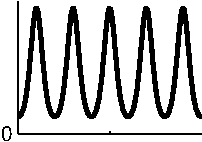
\includegraphics[width=\fwh,height=\fwb]{figures/structure_examples/per_kernel}} &  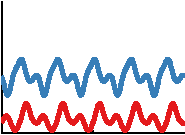
\includegraphics[width=\fwb,height=\fwh]{figures/structure_examples/per_kernel_draws} & 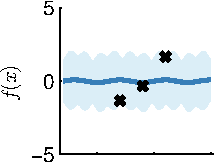
\includegraphics[width=\fwb,height=\fwh]{figures/structure_examples/per_kernel_post} \\
periodic & \multicolumn{2}{c}{repeated structure} \\ \midrule
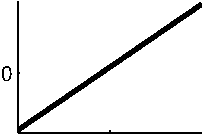
\includegraphics[width=\fwb,height=\fwh]{figures/structure_examples/lin_kernel} &  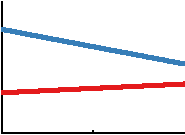
\includegraphics[width=\fwb,height=\fwh]{figures/structure_examples/lin_kernel_draws} & 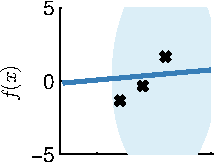
\includegraphics[width=\fwb,height=\fwh]{figures/structure_examples/lin_kernel_post} \\
linear & \multicolumn{2}{c}{linear functions} \\ \midrule
\rotatebox{90}{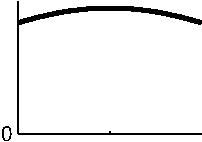
\includegraphics[width=\fwh,height=\fwb]{figures/structure_examples/longse_kernel}} &  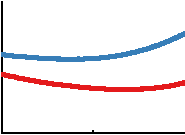
\includegraphics[width=\fwb,height=\fwh]{figures/structure_examples/longse_kernel_draws} & 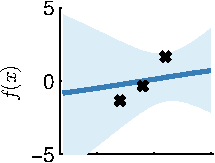
\includegraphics[width=\fwb,height=\fwh]{figures/structure_examples/longse_kernel_post} \\
long-length SE & \multicolumn{2}{c}{slowly changing}
\end{tabular}
\end{figure}
